\documentclass{article}
\usepackage[hmargin=0.65in, vmargin=0.65in]{geometry}
\usepackage[utf8]{inputenc}
%% \usepackage{indentfirst}
\usepackage{listings}
\usepackage{xcolor}
\usepackage{hyperref}
\hypersetup{
    colorlinks=true,
    linkcolor=blue,
    filecolor=magenta,      
    urlcolor=cyan
    }
\usepackage{graphicx}
\graphicspath{ {./images/} }


\title{CS 470 Homework 3}
\author{Niki Vasan}
\date{March 16th, 2023}

\begin{document}

\maketitle

\textbf{Collaboration Statement:} I pledge to abide by the Emory honor code. I used the following sources as a reference in the completion of this assignment and did not collaborate with any peers on the implementation of my code. 
\begin{enumerate}
    \item \href{https://github.com/Theob0t/Medium/blob/master/K-means-implementation.ipynb}{Clustering Visualization Implementation}: I used this source to help me visualize the clusters
    \item Course Textbook
\end{enumerate} 

\paragraph{\textbf{Approach:}} The two datasets I chose were the Iris dataset and the Wine Quality (red) dataset from the UCI Machine Learning Repository. Because both of these datasets consist only of quantitative variables, I chose to normalize the features using sklearn's Standard Scaler as a pre-processing step. This is important because I also chose the Euclidean Distance as my distance metric, which is sensitive to feature scale.  

For my implementation, I split the algorithm into a train and predict function, with some helper functions to calculate distances, normalize the features and visualize the clusters or evaluate metrics. In the train function, I separate the data into training and testing data and then I normalize the data. The predict function implements the algorithm itself. I store the centroids, k value and max iterations as class attributes. I first randomly initialize the centroids. I then iteratively assign the points to a centroid and update the centroids by taking the numerical mean of all the points in its assigned cluster.

One important decision was how to deal with empty clusters, whose mean would automatically result in NaN. Instead of aborting the algorithm at this point, I chose to keep the previous centroid of the same index as the current centroid (e.g. if C1 = [1,2,3] and C2 = [5,6,NaN], then C2 = [5,6,3]). The termination condition is if the centroids are the same as the previous centroids or if the maximum number of iterations is reached (1000).

\paragraph{\textbf{Results (Iris Dataset):}} 
Here is a visualization of the clusters at k=3 and n-iterations = 3. I chose k=3 because in this dataset, we actually have access to the class labels, and there are three class labels in the original dataset (Versicolor, Setosa, Virginica). 

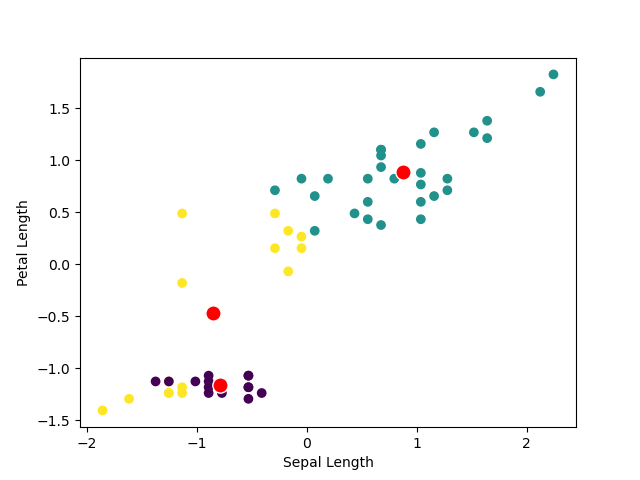
\includegraphics[scale=0.6]{Visualize-Iris.png}

I also looked at how the within-cluster SSE and Silhouette coefficient with respect to k. 

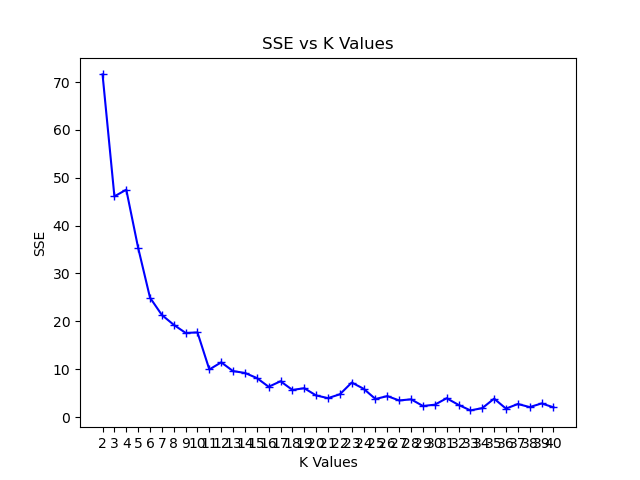
\includegraphics[scale=0.6]{SSE-plot-iris.png}

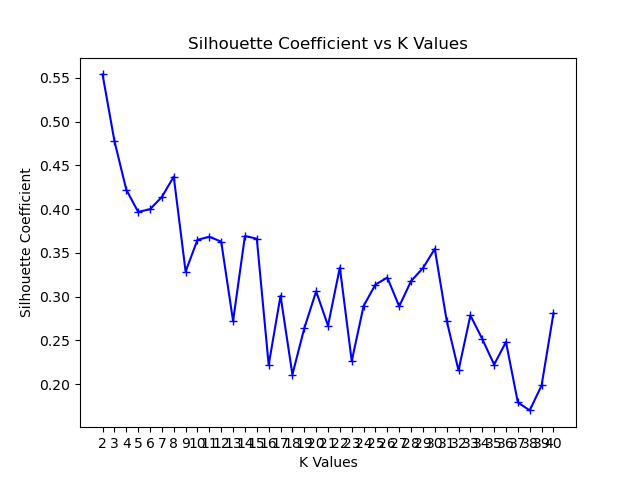
\includegraphics[scale=0.6]{Silhouette-plot-iris.png}

We can see that the SSE decreases as the number of clusters increases. The elbow shape of the curve is not very accentuated, however. This is most likely due to the random initialization of the centroids. This may results in empty/less dense clusters, which can skew the SSE and the Silhouette Coefficient.

\paragraph{\textbf{Results (Wine Dataset):}} 
Here is a visualization of the clusters at k=6 and n-iterations = 36. I chose k=6 because in this dataset, we also have access to the class labels, which is the wine quality score ranging from 3-8. 

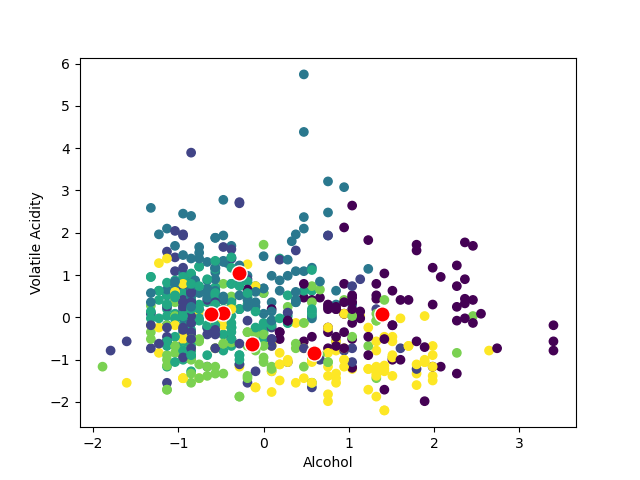
\includegraphics[scale=0.4]{Visualize-Wine.png}

I again looked at how the within-cluster SSE and Silhouette coefficient with respect to k. 

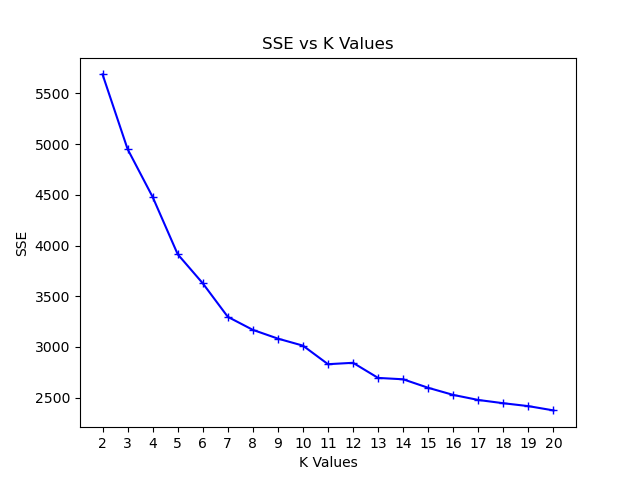
\includegraphics[scale=0.6]{SSE-plot-wine.png}

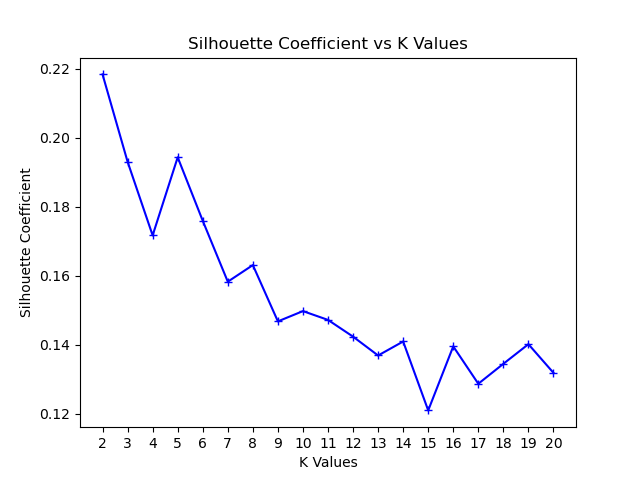
\includegraphics[scale=0.6]{Silhouette-plot-wine.png}

The silhouette coefficient is very low and the SSE values are very high for this dataset. This may imply that the data is very sparse, which seems reasonable given that I didn't do any feature selection or PCA to reduce the feature space, which consists of around 8 features.

\paragraph{\textbf{Insights and Conclusions:}} This assignment was interesting, because while the algorithm is conceptually simple, there are some things that need to be taken into consideration that can impact your code. These things include the initialization of centroids, how you handle empty clusters, the data structures used to store the data points and respective clusters, etc. In future implementations of this algorithm, I might be more intentional about the intialization of the centroids, and choose different data structures that are easier to work with for me personally (e.g. numpy arrays versus pandas dataframes).

\end{document}
